\documentclass[aspectratio=169,11pt]{beamer}
\usetheme{default}\usecolortheme{seagull}
\setbeamertemplate{navigation symbols}{}
\setbeamertemplate{footline}{\hfill{\scriptsize\color{muted}\insertframenumber/\inserttotalframenumber}\hspace{0.4cm}\vspace{0.2cm}}
\setbeamertemplate{itemize items}{\textendash}
\usepackage{fontspec}\setmainfont{TeX Gyre Pagella}\usefonttheme{serif}
\usepackage{booktabs,xcolor,graphicx,amsmath}
\definecolor{ink}{HTML}{1F1F1F}\definecolor{muted}{HTML}{6B6B6B}\definecolor{accent}{HTML}{8B1A1A}
\setbeamercolor{normal text}{fg=ink}\setbeamercolor{frametitle}{fg=ink}\setbeamercolor{title}{fg=ink}
\setbeamerfont{frametitle}{size=\large,series=\bfseries}\setbeamerfont{title}{size=\LARGE,series=\bfseries}
\setbeamersize{text margin left=1.1cm,text margin right=1.1cm}
\newcommand{\muted}[1]{{\color{muted}#1}}
\newcommand{\acc}[1]{{\color{accent}#1}}
\newcommand{\lead}[1]{\vspace{0.3em}{\large #1}\vspace{0.8em}}
\title{Age at Exposure to Violence}
\subtitle{Assessment of the Colombia design}
\author{Job market paper, idea 1}
\date{\muted{October 2026}}
\begin{document}
\begin{frame}[plain]\titlepage\end{frame}

%% 1
\begin{frame}{The idea}
\lead{Does the effect of violence on adult human capital depend on the age at which the child is exposed?}
\begin{itemize}
\item Setting: Colombian paramilitary violence, 1997--2006. Entry staggered across municipalities, a ceasefire in December 2002, 38 bloc demobilizations between 2003 and 2006, zero paramilitary victims after 2007.
\item Variation: children born in the same municipality were of different ages when the violence ended.
\item Outcomes: schooling, employment, earnings at ages 20--36 (GEIH), with municipality of birth.
\item Mechanism: household channel (caregiver stress, displacement) versus the child's direct exposure.
\end{itemize}
\end{frame}

%% 2
\begin{frame}{What we would have estimated}
\begin{equation*}
Y_{imc} = \sum_{a} \beta_a\, \text{Years exposed}^{a}_{mc} + \mu_m + \lambda_{c} + \text{trend}_{d(m)}(c) + \varepsilon_{imc}
\end{equation*}
\vspace{0.3em}
\begin{itemize}
\item $a$ = in utero, early childhood, preschool, primary, high school.
\item $\mu_m$: municipality-of-birth fixed effects. $\lambda_c$: year-of-birth fixed effects. Province trends.
\item Validity: violence before conception must have no effect.
\end{itemize}
\vspace{1em}
\acc{This is, line by line, equation (3) of León (2012, \emph{JHR}).}
\end{frame}

%% 3
\begin{frame}{The question is already well covered}
\footnotesize
\setlength{\tabcolsep}{4pt}
\begin{tabular}{@{}lll@{}}
\toprule
\textbf{Paper} & \textbf{Shock} & \textbf{Age windows} \\
\midrule
Bundervoet, Verwimp and Akresh (2009, \emph{JHR}) & Burundi civil war & months of exposure \\
Akresh, Bhalotra, Leone and Osili (2012, \emph{AER P\&P}) & Biafran war & birth to adolescence \\
León (2012, \emph{JHR}) & Shining Path, Peru & in utero to high school \\
Akbulut-Yuksel (2014, \emph{JHR}) & WWII bombing, Germany & school age \\
Singhal (2019, \emph{JDE}) & US bombing, Vietnam & early life \\
Duque (2024, \emph{JCR}) & Colombia, 1980s homicides & in utero to adolescence \\
Akbulut-Yuksel, Tekin and Turan (2025, \emph{JHR}) & WWII bombing, Germany & $\le 5$ vs 6--10 \\
\bottomrule
\end{tabular}
\vspace{1em}

Same design in all of them: birth location $\times$ cohort, fixed effects, exposure by age window. A fourth or fifth paper of this kind is not a job market paper.
\end{frame}

%% 4
\begin{frame}{The standard design just failed its replication}
\lead{Huaroto, Gonzales and Pacheco (2026, \emph{JHR}): León (2012) with the full-count census.}
\begin{itemize}
\item Same equation, same controls; 7 million observations instead of 139,000.
\item Violence \emph{before conception} has significant effects: the parallel pre-trends assumption fails.
\item Only the in-utero effect survives Rambachan and Roth (2023, \emph{REStud}) bounds.
\item Cause: where violence arrives is correlated with historical determinants of human capital. The cross-sectional variation is not exogenous.
\end{itemize}
\vspace{0.6em}
With our equation we would be proposing a design that has just been shown not to identify the age gradient it claims.
\end{frame}

%% 5
\begin{frame}{Our own data say the same}
\begin{center}
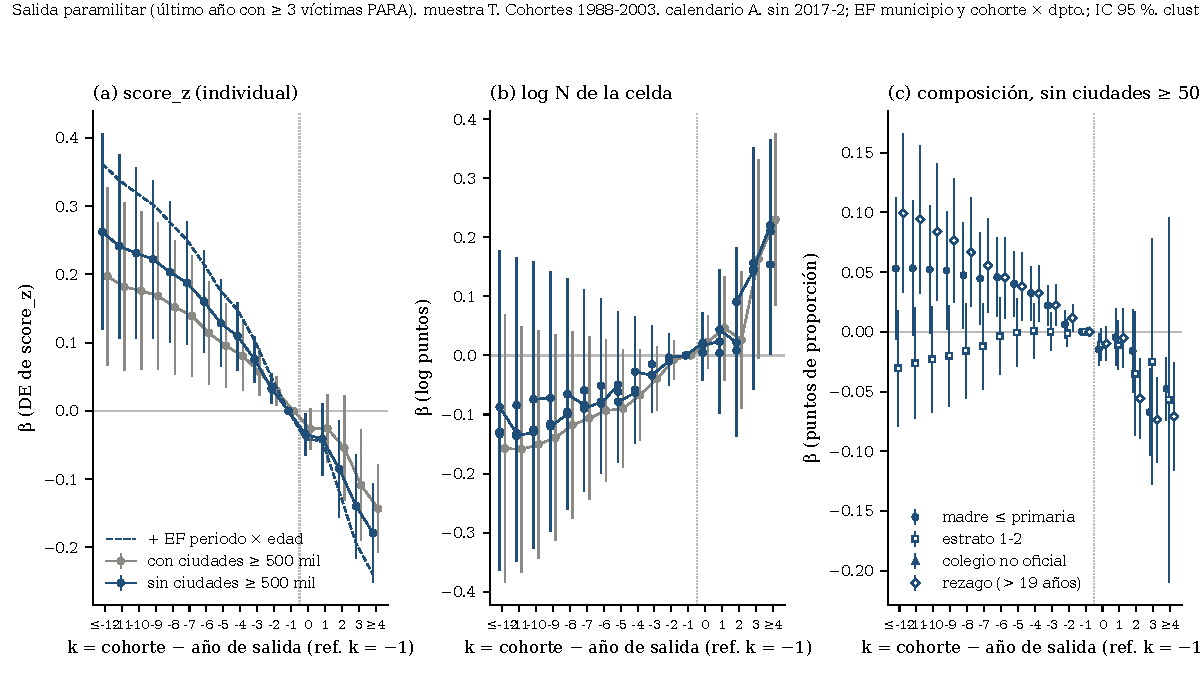
\includegraphics[height=0.52\textheight,page=1]{fig8_event_study_salida.pdf}
\end{center}
\small
Saber 11, 3.2 million test takers, cohorts relative to the municipal end of violence. No break at the end: a monotone cohort trend, with composition and the number of test takers moving in parallel. The pre-conception placebo is significant on both the violence and the displacement clocks.
\end{frame}

%% 6
\begin{frame}{Migration makes exposure endogenous, and no public data fix it}
\begin{itemize}
\item In affected municipalities the median share of population displaced in 1997--2010 is 23\%.
\item Exposure depends on whether the household stays and when it leaves; leaving is a different treatment.
\item Municipality of birth fixes the location but not the problem: the intention-to-treat effect is a mixture of violence, displacement and the selection of who leaves, with weights we cannot recover.
\item Separating channels needs individual migration histories linked to outcomes. They exist only in restricted linked records (ICFES, UARIV, PILA) with no access protocol.
\end{itemize}
\end{frame}

%% 7
\begin{frame}{The one escape route, and why it is not enough}
\lead{Use the \emph{end} of violence, set by a national negotiation calendar, as the source of variation.}
\begin{itemize}
\item It is a different, plausibly more exogenous source than the arrival of violence. It is the only new ingredient.
\item But 70\% of exits fall within eighteen months (July 2004 to December 2005): little variation in the age at the end.
\item Cohorts born after the end are not yet adults; with current data they exist in 28 municipalities.
\item And the estimating equation would still be the 2012 one: two-way fixed effects with a continuous, staggered dose. Everything the recent difference-in-differences literature warns against.
\end{itemize}
\end{frame}

%% 8
\begin{frame}{Assessment}
\begin{itemize}
\item \textbf{Question:} answered several times; its best-known answer has just been overturned, but not by us.
\item \textbf{Design:} 2012 vintage; fails the one validity test that matters, in Peru and in our own exploratory data.
\item \textbf{Mechanism:} not identifiable without linked individual records we do not have.
\item \textbf{As formulated:} an incremental age-gradient paper with a 2012 design. Not viable.
\end{itemize}
\vspace{0.8em}
\acc{Viable only if reformulated around a question that is actually open.}
\end{frame}

%% 9
\begin{frame}{The open question, and what we keep}
\lead{Is the long-run damage of violence prenatal or postnatal?}
\begin{itemize}
\item After the 2026 replication, only the in-utero effect is credible. Whether exposure after birth matters at all is unknown.
\item The dated end of paramilitary violence separates children exposed only in utero from those also exposed in infancy or preschool, within the same municipality of birth, with a source of variation set by a national negotiation calendar.
\end{itemize}
\vspace{0.4em}
\textbf{What we keep.}
\begin{itemize}
\item A municipality $\times$ month $\times$ perpetrator panel of victims, 1985--2015 (CNMH), with entry, peak and exit dated for 451 municipalities.
\item A displacement panel by municipality and year (RUV).
\item A working pipeline for 9 million Saber 11 records with date and place.
\end{itemize}
\end{frame}
\end{document}
